\documentclass[main.tex]{subfiles}
\section{Pure parabolic model problem}

In this section we shall study and analyze two different approaches for solving parabolic differential equations. Concretely we will focus on the heat diffusion problem, which can be modeled by the following partial differential equation and its initial and boundary conditions.

\begin{equation}
\begin{aligned}
u_t = \kappa u_{xx} \\
u(x,0) = \eta (x) \\
u(0,t) = g_L (t) \\
u(0,t) = g_R (t)
\end{aligned}
\end{equation}

The first thing we should notice is that, a part from having the usual spatial dependence, the equation also describes how the heat distribution evolves in time. Hence, if we want to solve this equation numerically we need to discretize both time and space, which means that the solution will be represented by a two dimensional grid.

\subsection{Matlab implementation of the $\theta$-scheme}

Applying euler approximation to the time derivative and the second order central finite difference to the right hand side in equation \ref{eq:diffusion}, an explicit scheme is obtained.

\begin{equation}
\frac{U_i^{n+1} - U_i^n}{k} = \frac{\kappa}{h^2}(U_{i-1}^n - 2 U_i^n + U_{i+1}^n)
\label{eq:scheme}
\end{equation}

where $h$ and $k$ represent the distance between two grid points in space and time respectively.

A more general scheme for solving this problem can be formulated as:

\begin{equation}
\frac{U_i^{n+1} - U_i^n}{k} = \frac{\kappa}{h^2}((1-\theta)(U_{i-1}^n - 2 U_i^n + U_{i+1}^n) + \theta(U_{i-1}^{n+1} - 2 U_i^{n+1} + U_{i+1}^{n+1})
\label{eq:genscheme}
\end{equation}
where $0 \leq \theta \leq 1$

It is easy to see that when $\theta = 0$ equation \ref{eq:genscheme} is equivalent to \ref{eq:scheme}. However for any other value of $\theta$ the scheme becomes implicit but also more accurate. 
%% TODO: [FIXES] Make sure to remove this before handing in
[[[[The solution at one point in space relies on both its spatial neighbors at the current time and at the previous.]]]!!!

The scheme takes the form of system of equations which can be written in matrix form as:

\begin{equation}
(I - \theta \mu A_0) \mathbf{u}^{n+1} = (I + (1-\theta)\mu A_0) \mathbf{u}^n + (\mathbf{g}^{n+1} - \mathbf{g}^n)
\end{equation}

\begin{equation}
A_L \mathbf{u}^{n+1} = A_E \mathbf{u}^n + (\mathbf{g}^{n+1} - \mathbf{g}^n)
\label{eq:matrixform}
\end{equation}

where $I$ is the identity matrix and $u^n$ and $g^n$ are vectors of the form

\begin{equation}
\mathbf{u^n} = 
\begin{bmatrix}
U_0^n && U_1^n && ... && U_{M-1}^n && U_{M}^n
\end{bmatrix}^T
\qquad
\mathbf{g^n} = 
\begin{bmatrix}
g_L^n && 0 && ... && 0 && g_R^n
\end{bmatrix}^T
\end{equation}

while $A_0$ is a matrix of dimensions $(M+1) \times (N+1)$ of the form

\begin{equation}
A_0 = \begin{bmatrix}
0 && 0 \\
1 && -2 && 1 \\ 
&& \ddots && \ddots && \ddots \\
&& && 1 && -2 && 1
\end{bmatrix}
\end{equation}

Equation \ref{eq:matrixform} is nothing but a system of ordinary differential equations and thus, the solution at a given time can be obtained by inverting the tridiagonal matrix in the left hand side. Consequently, using a loop the global solution can be computed sequentially at every point in the time grid.

The code snippet below shows the implementation of this scheme in MATLAB where the function given by equation 2 in the assignment specifications is used to compute the initial and boundary conditions.

\lstinputlisting{../Ex1/parabolicSolver.m}

Figure \ref{fig:solution} represents the solution at different points in time. It is easy to see in the graphs how the higher frequencies in the heat wave are damped quickly while the lower ones remain longer.

\begin{figure}[H]
    \centering
    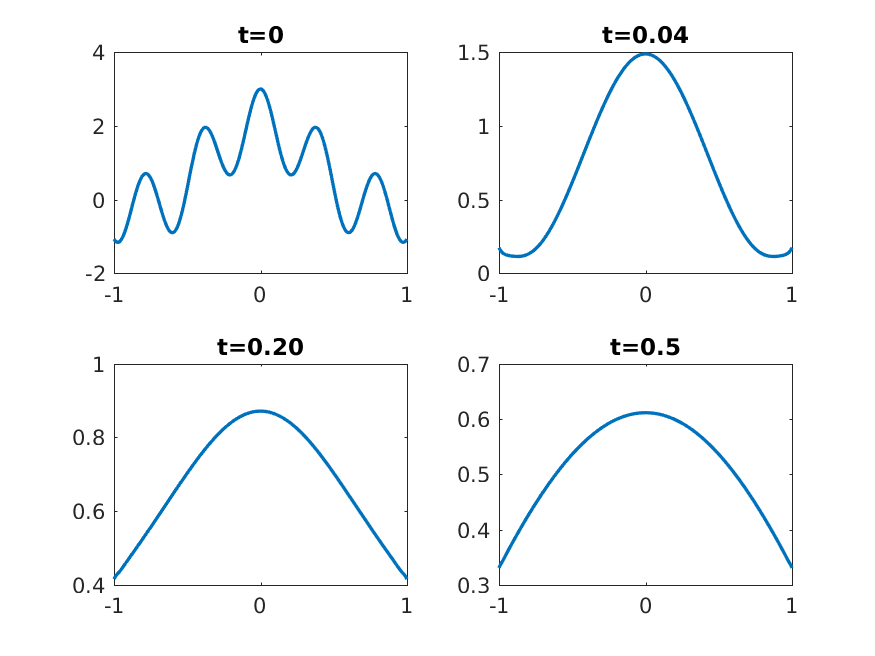
\includegraphics[width=\textwidth]{../Figures/sol}
    \caption{Solution of the heat diffusion equation at different points in time using the $\theta$-scheme}
    \label{fig:solution}
\end{figure}
\subsection{Analytical analysis $\theta = 0$}

Once the the scheme for solving the problem numerically has been built, it might be interesting to make an analysis on the system and draw some conclusions about how large the grid should be for the solver to be stable, what is its order of consistency or under what circumstances it satisfies the discrete maximum principle.


\subsubsection{Consistency}

As mentioned, for $\theta = 0$ equation \ref{eq:genscheme} corresponds to the explicit forward time and central space scheme. We first check that the finite difference approximation is consistent, that is, the local truncation error approaches to 0 as the grid size increases.

\begin{equation}
\tau(x,t) = \frac{u(x,t+k)-u(x,t)}{k} - \frac{\kappa}{h^2}(u(x-h,t) - 2 u(x,t) + u(x+h,t))
\label{eq:LTE}
\end{equation}

by applying the Taylor series expansions about u(x,t)

\begin{equation}
\tau(x,t) = \left(u_t + \frac{1}{2}k u_{tt} + \frac{1}{6}k^2u_{ttt} + ...\right) - \kappa \left(u_xx + \frac{1}{12}h^2 u_{xxxx} + ...\right)
\end{equation}

and since we know that $u_t = \kappa u_xx$ and $u_tt = \kappa^2 u_xx$ then 

\begin{equation}
\tau(x,t) = \left(\frac{\kappa^2}{2} k - \frac{\kappa}{12}h^2 \right)u_{xxxx} + \mathcal{O}(k^2 + h^4)
\end{equation}

where the dominant term depends on $k$ and $h^2$ which means that the scheme is consistent of order $\mathcal{O}(k + h^2)$. 

Besides, for  $\mu = 1/6$

\begin{equation}	
\tau(x,t) = h^2\left(\frac{\kappa}{12} - \frac{\kappa}{12} \right)u_{xxxx} + \mathcal{O}(k^2 + h^4)
\label{eq:order}
\end{equation}

the first term in the right hand side of equation \ref{eq:order} disappears and the order becomes $\mathcal{O}(k^2 + h^4)$.

\subsubsection{Stability}

Secondly, in order to find the stability of the method we need to check when the eigenvalues of the matrix $A_E$ in the right hand side of equation \ref{eq:matrixform} lie within the unit circle.

According to 2.23 in Randall Leveque the eigenvalues of $A_0$ are given by

\begin{equation}
\lambda_p =  2(\cos(p \pi h) - 1) \qquad \mathrm{for} \qquad p = 1,2, ..., m
\label{eq:eig}
\end{equation}

Therefore, the system would be absolutely stable when $|1+\mu \lambda_p| \leq 1$ and since the smallest $\lambda_p$ is approximately $-4$ we have that the region is defined by:

\begin{equation}
-2 \leq -4 \mu \leq 0
\end{equation}

which means that for the system to be stable the following relation must be satisfied

\begin{equation}
\frac{\kappa k}{h^2} \leq \frac{1}{2}
\end{equation}

\subsubsection{Convergence}

According to theorem 9.2 and definition 9.1 in R.L. a system of the form (9.16) is convergent if there is a constant $C_t > 0$ such that 

\begin{equation}
||B(k)^n|| \leq C_t
\end{equation}  

in our case

\begin{equation}
B(k) =  A_E = I + \mu A_0 
\end{equation}

We already showed in section 1.2.2 that for $\mu \leq 1/2$ the eigenvalues of $A_E$ lied within the unit circle and hence, $||A_E|| \leq 1$, which means that for this choice of $\mu$ the system is both Lax-Richtmyer stable and convergent.


\subsubsection{Discrete Maximum Principle}

The discrete maximum principle states that if the solution is bounded from above and below by the most extreme values of the initial and boundary conditions then, as long as the conditions are consistent and smooth, it will converge uniformly.

According to Lecture 21 slide 17 the $\theta$-scheme will satisfy the discrete maximum principle when:

\begin{equation}
\mu(1-\theta) \leq \frac{1}{2}
\end{equation}

and in this case since $\theta = 0$

\begin{equation}
\frac{\kappa k}{h^2} \leq \frac{1}{2}
\end{equation}

which is consistent with the stability criteria.

%% TODO: [FIXES] Possibly a mistake in the title
\subsection{Analytical analysis $\theta = 1/2 + h^2/(12k\kappa)$}

\subsubsection{Consistency}

According to what we saw when developing the $\theta$-scheme we should expect a higher order for this particular choice of  $\theta$ than in the previous case. The LTE is in this case

\begin{multline}
\tau (x,t) = \frac{u(x,t+k)-u(x,t)}{k} - \frac{\kappa}{h^2}\Biggl(\left(\frac{1}{2} - \frac{h^2}{12k\kappa}\right) (u(x-h,t) - 2u(x,t) + u(x+h,t)) + \\ \left(\frac{1}{2} + \frac{h^2}{12k\kappa} \right) (u(x-h,t+k) - 2u(x,t+k) + u(x+h,t+k))\Biggl)
\end{multline}

by taking Taylor expansions in the expression above

\begin{multline}
\tau (x,t) = \left(u_t + \frac{1}{2}k u_{tt} + \frac{1}{6}k^2u_{ttt} + ...\right) - \frac{\kappa}{h^2}\Biggl( \left(\frac{1}{2} - \frac{h^2}{12k\kappa} \right) (h^2 u_{xx} + \frac{1}{12}h^4 u_{xxxx} + ...)  + \\ \left(\frac{1}{2} + \frac{h^2}{12k\kappa} \right) (h^2 u_{xx} + \frac{k^3}{6}u_{ttt}+...)\Biggl)
\end{multline}

and since we know that $u_t = \kappa u_{xx}$, $u_{tt} = \kappa^2 u_{xxxx}$ and $u_{xxt} = \kappa u_{xxxx}$ then

\begin{equation}
\tau (x,t)  = \left(\frac{\kappa h^2}{2} - \frac{h^2}{24}\right) u_{xxxx} + \left(\frac{k^2}{6} + \frac{k^3}{6}\right) u_{ttt} \quad ...
\end{equation}

where the dominant term depends on $k^2$ and $h^2$ which means that the scheme is consistent of order $\mathcal{O}(k^2 + h^2)$. 

\subsubsection{Stability}

Following the same approach as before the eigenvalues of $B = A_L^{-1}A_E$ should lie inside the unit circle.

\begin{equation}
\lambda_B = \frac{1+ \theta \mu \lambda_p}{1 - \theta \mu \lambda_p }  = \frac{1 + (\frac{1}{2} \mu + \frac{1}{12}) \lambda_p}{1 - (\frac{1}{2} \mu + \frac{1}{12}) \lambda_p}
\end{equation}

where $\lambda_B$ is given by equation \ref{eq:eig} and $\mu = \kappa k / h^2$. We know that $\lambda_p$ is strictly negative and since for the scheme to be stable $|\lambda_B| \leq 1$, we need $\mu$ to be positive. Which means that the system will be stable for any choice of $h > 0$ and $k > 0$.

\subsubsection{Convergence}

Again, a system of the form (9.16) is convergent if it is Lax-Richtmyer stable. We have proved in the previous section that the eigenvalues of $B$ are within the unit circle for any positive choice of the step size. Hence, in this case

\begin{equation}
||B(k)|| \leq 1
\end{equation}  

for any $k > 0$ and $h > 0$.

\subsubsection{Discrete Maximum Principle}

Again, the $\theta$-scheme will satisfy the discrete maximum principle when:

\begin{equation}
\mu(1-\theta) \leq \frac{1}{2}
\end{equation}

and in this case since $\theta = \frac{1}{2} + \frac{1}{12 \mu}$

\begin{equation}
\frac{\kappa k}{h^2} \leq \frac{5}{6}
\end{equation}



\subsection{Numerical evaluation}

After deriving the analytical expressions, we shall check that the rates and the conditions obtained are satisfied in reality. To do so, we insert the solver implemented in MATLAB in a loop where we vary the time and space grids accordingly so that the system remains within the stability region and satisfies both the convergence criteria and the discrete maximum principle.

For the choice of $\theta = 0$, figure \ref{fig:conv1} represents the variation of the LTE when changing the size of  $h$ and $k$. In this case, we set the value of $k$ to be equal to $\frac{h^2}{2}$ so that the eigenvalues of the system lie within the unit circle. The dashed lines, which are the theoretical order of the system ($\mathcal{O}(h^2)$ and $\mathcal{O}(k)$), can be thought as an upper bound for the empirical curves. It is easy to see that in both comparisons the slope of the LTE in logarithmic scale is greater than the slope of the help lines.

\begin{figure}[H]
    \centering
    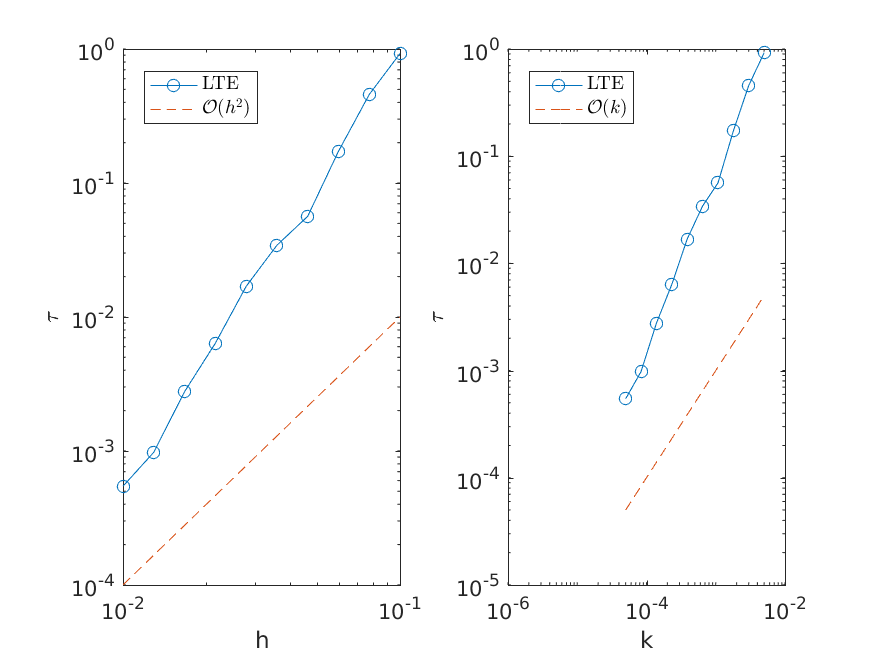
\includegraphics[width=\textwidth]{../Figures/c1}
    \caption{Local truncation error for different values of $h$ and $k$, $\mu = 1/2$ and $\theta = 0$ in logarithmic scale.}
    \label{fig:conv1}
\end{figure}


When $k = h^2/6$ the graph in figure \ref{fig:conv2} also reveals that the the local truncation error respects the theoretical limits of $\mathcal{O}(h^4)$ and $\mathcal{O}(k^2)$.

\begin{figure}[H]
    \centering
    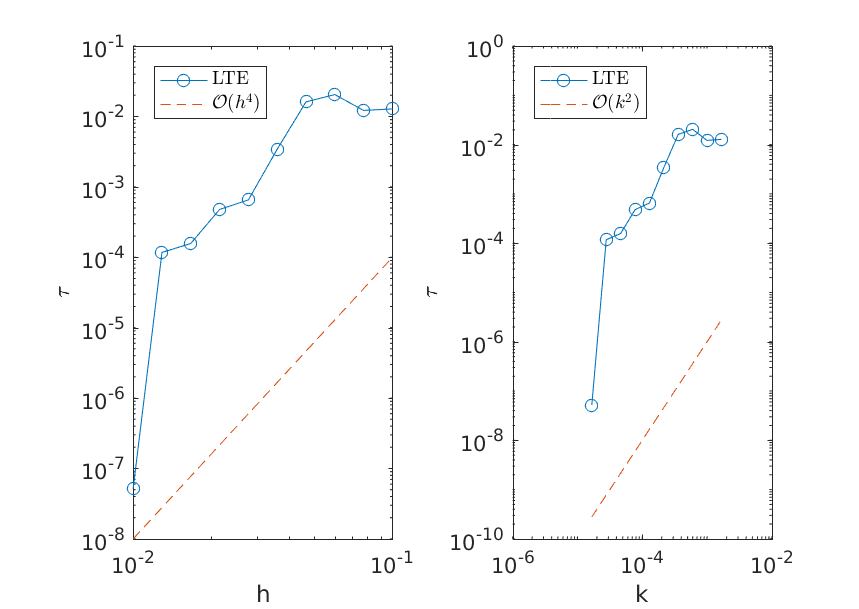
\includegraphics[width=\textwidth]{../Figures/c2}
    \caption{Local truncation error for different values of $h$ and $k$, $\mu = 1/6$ and $\theta = 0$ in logarithmic scale.}
    \label{fig:conv2}
\end{figure}
%% TODO: [FIXES] Broken reference here to fig:conv3
On the other hand, for the especial choice of $\theta = 1/2 + h^2/(12k\kappa)$ figure \ref{fig:conv3} also holds with what we found when we evaluated the scheme analytically in the previous section. Besides, in order to satisfy the discrete maximum principle $k$ was selected so that $\mu = 5/6$.

\begin{figure}[H]
    \centering
    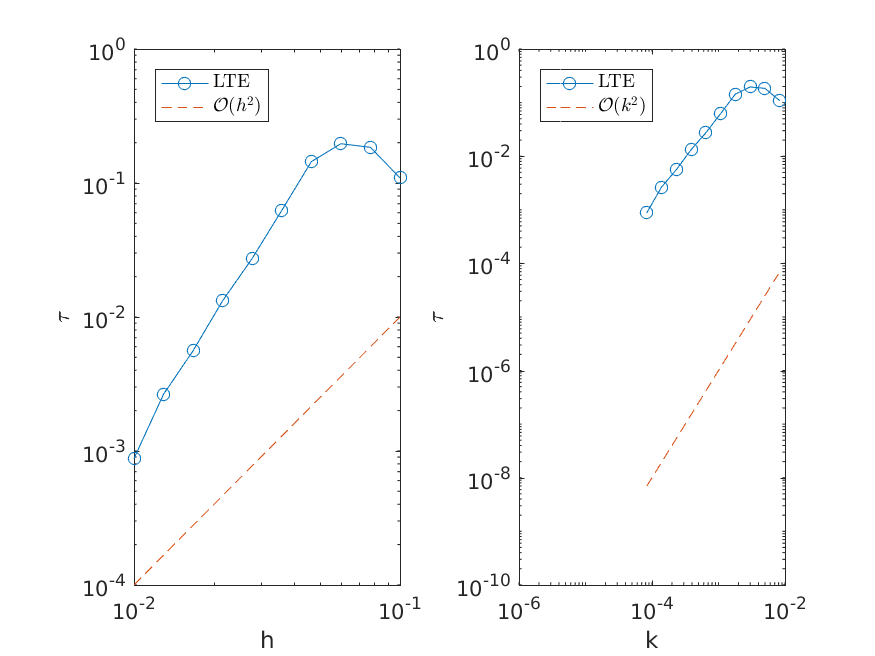
\includegraphics[width=\textwidth]{../Figures/c3}
    \caption{Local truncation error for different values of $h$ and $k$, $\mu = 5/6$ and $\theta = 1/2 + h^2/(12k\kappa)$ in logarithmic scale.}
    \label{fig:conv2}
\end{figure}
